\documentclass{article}

\usepackage[latin1]{inputenc}
\usepackage{pgfplots}
\usepackage{tikz}
\usetikzlibrary{arrows}

\pgfplotsset{compat=1.10}

\begin{document}
\pagestyle{empty}

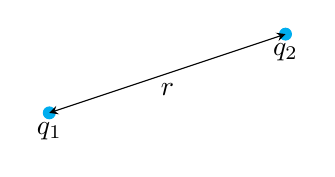
\begin{tikzpicture}[>=stealth]
	\draw[cyan, fill] (0, 0) circle [radius=0.075] node[black, below] {$q_1$};
	\draw[cyan, fill] (3, 1) circle [radius=0.075]  node[black, below] {$q_2$};

	\draw[<->, thin] (0, 0) -- (3, 1);
	\node[below] at (1.5, 0.5) {$r$}; 
\end{tikzpicture}

\end{document}